This chapter details the controller design of the model based controller. The performance of the controller is tested with the aid of a simulation model. In order to so, the pump characteristics need to be determined, as they have a major impact on the dynamics of the entire system. 


\section{Jacobian control}


The controller designed in this study includes jacobian information. Jacobian control is a widely used type of model-based controller for positioning classic robots. As mentioned in Chapter \ref{chap1}, jacobian controllers only use model information on velocity and position level. Thus, system dynamics are not used in this control law.


The Jacobian controller proposed is an adapted version of the one presented in \cite{MOOSAVIAN20071226}. This work shows that a computed torque controller can be approximated by a more straightforward control law involving the Jacobian transpose. This approximation holds if high enough control gains are used. This work only uses a proportional and derivative action to reduce the error. In order to remove the steady-state error, an integrator gain is added this controller. This Jacobian transposed control law is given by,


\begin{equation}
    \tau_{set} = \begin{bmatrix}J(\sigma,t)\end{bmatrix}^\top \Big(K_p e + K_i \int_0^t e \hspace{2pt} ds +  K_d \dot{e}\Big), 
    \label{eq:tau}
\end{equation}

where $\tau_{set} \in \mathbb{R}^2$ is the control input vector with control input moment and force. The Jacobian is determined with equation \ref{eq2:J}. Furthermore, $K_p,K_i and K_d \in \mathbb{R}^{2\times 2}$ are diagonal gain matrices. Here $K_p$ penalizes proportional to the error, $K_i$ contributes to the sum of the error over time, and $K_d$ penalized the error derivative. The error $e \in \mathbb{R}^2$ is defined as the difference between reference position and the actual position in the (x,y)-plane. Therefore not the entire Jacobian of dimension $6 \times 2$, but only the entries mapping modal coordinate velocity to linear velocity in x-y plane. As mentioned this Jacobian is space-time variant. Therefore, in the control law this Jacobian is calculated real-time based on the actual kinematic configuration of the actuator. 

The actual system does not allow to induce forces and moments directly. Therefore this control input should be mapped to pressure. This is done by the input mapping, as determined in Chapter \ref{chap3}. Based on the desired control input, a reference pressure can be formulated as,

\begin{equation}
    p_{ref} = H^{-1}\tau,
\end{equation}


where $p_{ref} \in \mathbb{R}^2$ is the reference pressure for each bellow. In order for this reference pressure to be reached a second controller is necessary. This low-level controller is used to set the input voltage that is supplied to the pumps.  The volt input is regulated via pulse width modulation (pwm). Since the Raspberry PI is equipped with a 12bit ADC (analog-digital converter), it is possible calculate the pwm input as, $\textit{pwm} = \frac{2^{12} V}{V_{max}} $, where $V_{max}$ is equal to 12 volt. This control law is given by,


\begin{equation}
    pwm_{set} = K_{pp}e_p \hspace{10pt} \text{with} \hspace{10pt} e_p = p_{ref} - p,
\end{equation}



where $PWM_{set}$ is the input voltage and $K_{pp} \in \mathbb{R}^{2\times 2}$ a diagonal gain matrix. Furthermore, $e_p$ is the pressure error, which is the difference between reference pressure and actual pressure. Observe that only a proportional action is used. The integral action of the jacobian controller will already ensure no steady-state error.


\section{Pump Dynamics}


\begin{theorem}
It is assumed that both air pumps have the equal pump characteristics
\end{theorem}


Besides soft robot actuator properties also the actuator properties need to be involved. To this end pump dynamics need to be determined. In the proposed control architecture, the high level Jacobian controller is accompanied by a lower level pressure controller. The reference pressure is determined by the Jacobian controller by some force to pressure mapping. To this end, the pump dynamics need to be determined. Initially, we solely determine the pump dynamics. Using this dynamics will result to poor performance once connected to the soft actuator. To suppress noise levels and provide capture the actual system dynamics the set-up is slightly adapted.

To determine the pump dynamics the pump is connected directly to the pressure sensor using a short flexible silicone hose. The pump is powered by an electric 12V DC motor, and uses membranes to create pressure. The pump characteristics are obtained by observing the systems response for various volt step inputs between 1 and 6 Volt. Although the pumps are able to operate at 12 Volt, only a maximum step input of 6V is possible for this set-up. The pressure sensor measures absolute pressures between 0 and 25 PSI, which is equivalent to a maximum of 172 kPa. Depending on weather conditions, the maximum theoretically measurable pressure is around 72 kPa. However, experiments have shown results up to 80 kPa are possible. The resulting step responses are shown in Figure (\ref{fig1:pump_dynamcis}).

\begin{figure}[H]
    \centering
    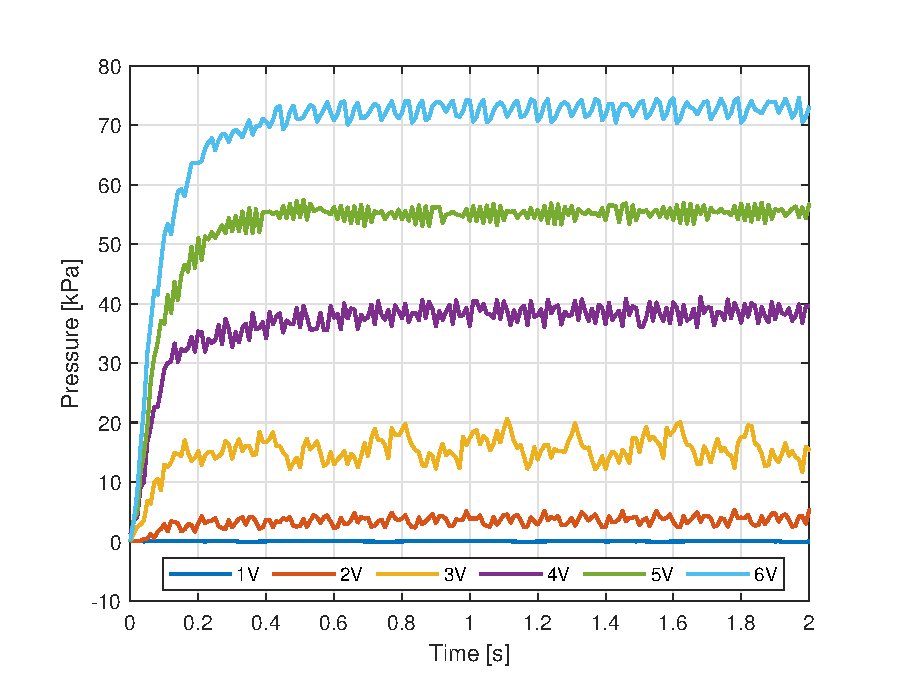
\includegraphics[width = 0.6\textwidth]{Figures/Chapter3/stepresponsdirect16V.eps}
    \caption{Step response for volt step input between 1V and 6V.}
    \label{fig1:pump_dynamcis}
\end{figure}

From Figure (\ref{fig1:pump_dynamcis}) multiple observations can be made. The step response indicates first order system behaviour as the pressure increase is proportional to the actual pressure. However, the steady-state pressure is not proportional to the input volt. The reason for this behaviour is friction. For 1 and 2 volt input static friction dominates, resulting in no to very small pressure increase.
At 3 volt the transition between dry and kinetic friction is observed. The first order system characteristic becomes more visible, although the pressure response is chattering. Furthermore, we see a rise time of comparable order for step inputs of 4V and above. After around 0.5 seconds the steady-state pressure is reached. For all step inputs oscillations are observed around the steady-state pressure. This phenomena is caused by the fact that there is almost no passive leakage from the small control volume. When the pump valves open and air is pressed into the system the air waves are created. For the step input of 5 volt the valve dynamics can be clearly seen, as the dense red spikes.

An improved pump model can be made by altering the set-up. To this end, the actuator and an air vessel are connected to the system. Previous research showed that adding an air vessel will reduce oscillatory behaviour, at the cost of bandwidth \cite{proper}. The air vessel will increase the control volume of the entire system. When the valves open and additional air is pressed in the system, the relative pressure change is smaller. Additionally, when the actuator expands the relative volume increase will also be smaller. This will cause the system to respond slower to a step input. Furthermore, the maximum achievable pressure is lower. The addition of air vessel and actuator will increase the passive leakage of the system.

For the adapted system the step response is determined for volt steps between 2 and 12 volt. The results are shown in Figure \ref{fig3:pump_dynamics_adapted}.

\begin{figure}[H]
    \centering
    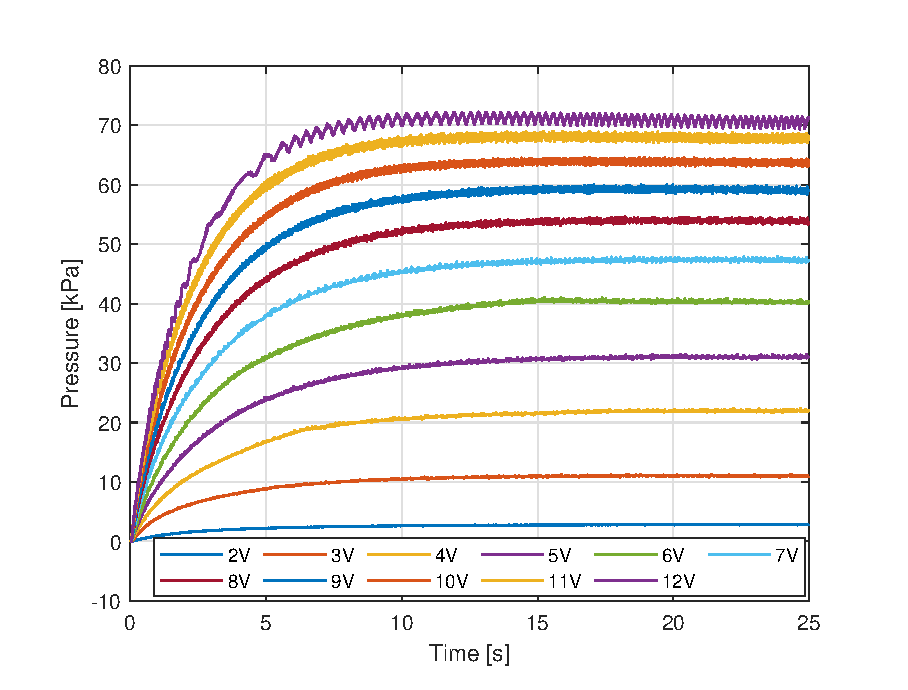
\includegraphics[width = 0.6\textwidth]{Figures/Chapter3/step212V.eps}
    \caption{Step response for volt step input between 2V and 12V for the system including air vessel and actuator.}
    \label{fig3:pump_dynamics_adapted}
\end{figure}


Based on the step responses of Figure (\ref{fig3:pump_dynamics_adapted}) we try to capture the pump dynamics in a model. The time response of a first order linear system responding to a step input is given by, 

\begin{equation}
    p(t,V) = K(1-e^{-t/\tau})V,
    \label{eq3:firstordermodel}
\end{equation}

where $p$ is the pressure at time $t$ in kPa. And constant DC gain $K$ [kPa/V] determines the maximum pressure, time constant $\tau$ [1/s] determines the growth rate of the exponential function. Furthermore, $V$ is the input volt. 

An attempt to fit the linear first order model of (\ref{eq3:firstordermodel}) did not result in an accurate description of the pump dynamics for all step inputs. Therefore an alternative description of the pump dynamics is proposed. In this description constant $K$ is replaced by a nonlinear function $K(V)$. Additionally, a linear function $\tau(V)$ is proposed. 

Based on (\ref{eq3:firstordermodel}) an indication of the gradient between constant $K$ and $V$ can be estimated. The steady-state pressure for each step is estimated by taken the mean over the last 10 seconds of the step response. This pressure is then divided by the corresponding volt input. A similar approach is done for determining time constant $\tau$. For a first order system it can be proven that this time constant is equal to time at which 63\% of the steady state value is reached. The corresponding relations for $K(V)$ and $\tau(V)$ are shown in Figure \ref{fig3:Kest} and Figure \ref{fig3:tauest}, respectively.

\begin{figure}[H]
\begin{minipage}[b]{0.48\linewidth}
\centering
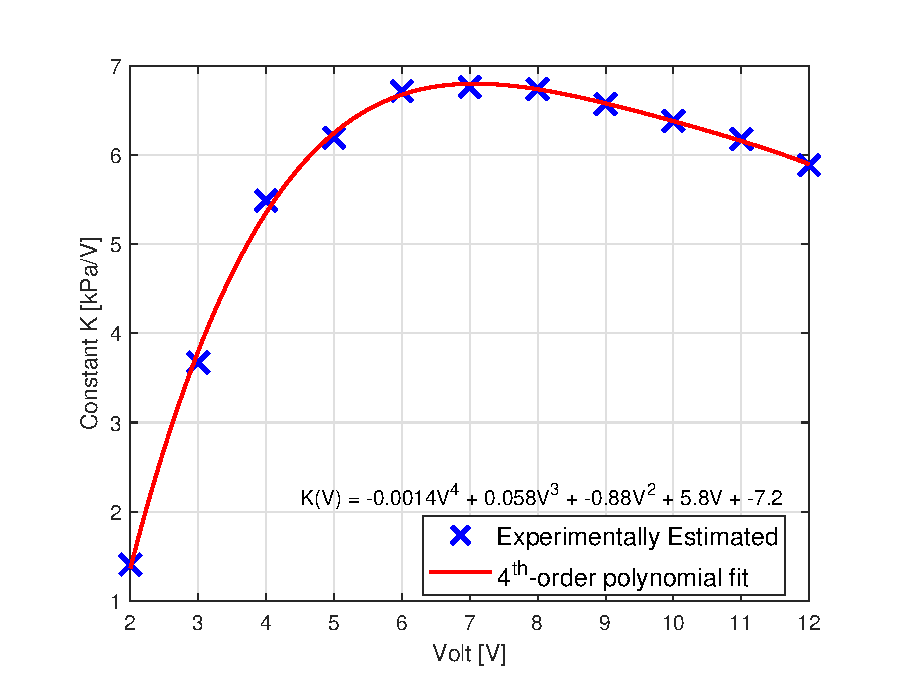
\includegraphics[width=\textwidth]{Figures/Chapter3/Kest.eps}
\caption{Experimental estimate of `constant' $K$ and fourth order fit.}
\label{fig3:Kest}
\end{minipage}
\begin{minipage}[b]{0.48\linewidth}
\centering
\includegraphics[width=\textwidth]{Figures/Chapter3/tauest.eps}
\caption{Experimental estimate of time `constant' $\tau$ and linear fit.}
\label{fig3:tauest}
\end{minipage}
\end{figure}

Figure (\ref{fig3:Kest}) shows a fourth-order polynomial fit to DC-gain $K$. For this fit all data samples were used. Figure (\ref{fig3:tauest}) shows that the estimated time constants for 2 and 3 volt do not follow linear trend line from 4 volt and above. Therefore, in determining the time `constant' $\tau$, only data point from 4 volt onward are used. A possible explanation for these outliers is the friction acting at these voltage inputs, and are therefore not reliable. Furthermore, from a physical point of view, relating time constant $\tau$ to input $V$ is doubtful. Instead, one would prefer defining $\tau$ based on system parameters. However, from a modelling point of view, this method allows to capture the actual model dynamics fairly accurate.

The obtained measurement fits for $K$ and $\tau$ can be substituted in (\ref{eq3:firstordermodel}) resulting in an expression as,

\begin{equation}
    p(t,V) = K(V)(1-e^{-t/\tau(V)})V.
    \label{eq3:firstodernonlinearmodel}
    \end{equation}

The derived first order model of (\ref{eq3:firstodernonlinearmodel}) can be plotted against the experimental results of Figure (\ref{fig3:pump_dynamics_adapted}), this is shown in Figure (\ref{fig3:expvsfitpres}).

\begin{figure}[H]
    \centering
    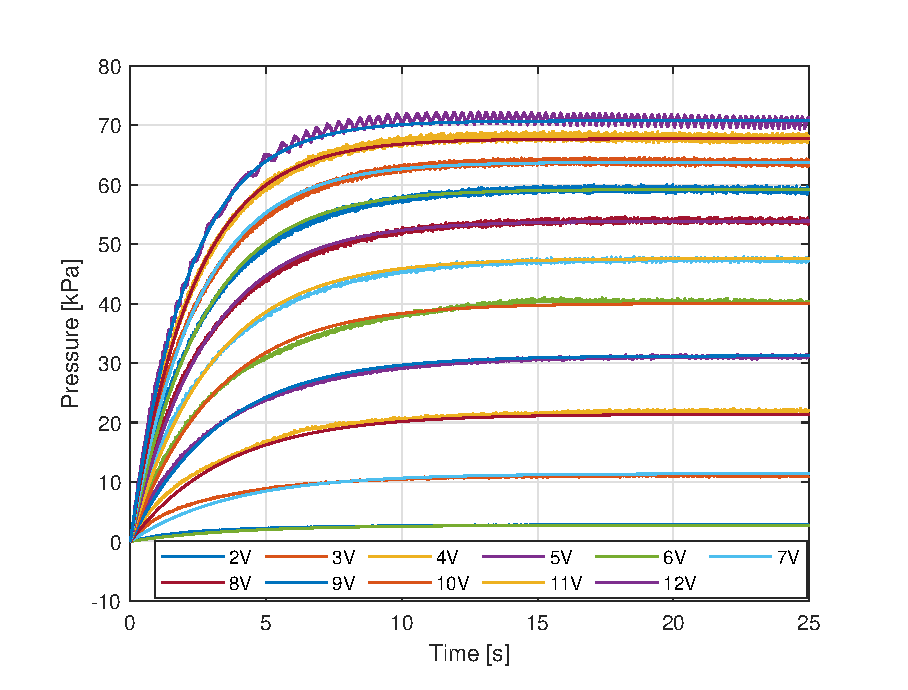
\includegraphics[width = 0.8\textwidth]{Figures/Chapter3/expfit.eps}
    \caption{Experimental results and the derived nonlinear pressure model.}
    \label{fig3:expvsfitpres}
\end{figure}

Above figure shows that the derived model captures the behaviour of the system with actuator and air vessel accurately. The steady-state pressure is close to the experimental value for all volt step inputs. As expected, the rise time for the 1 and 2 volt step inputs are not captured that well by this model.



\section{Controller in Simulation}

A simplified dynamic model is derived in an effort to capture the dynamics of the soft manipulator. It is assumed that the dynamics of the system can be formulated as, 

\begin{equation}
    M(q)\Ddot{q} + C\dot{q} + K(q)q = u \hspace{10pt} \text{with} \hspace{10pt} u = Hp
\end{equation}

which resembles a non-linear mass-spring-damper system. Here, $M(q)  \in \mathbb{R}^{n\times n}$ is a non-linear mass matrix, $C   \in \mathbb{R}^{n\times n}$ a linear damping matrix, and $K(q)   \in \mathbb{R}^{n\times n}$ a non-linear stiffness matrix. Matrix $H   \in \mathbb{R}^{2\times 2}$ maps input pressure $p$ to forces and moments $u$.

Above dynamic model allows for numeric solving by reformulating the model to a second order state-space formulation as,

\begin{equation}
     \begin{bmatrix} \dot{x}  \end{bmatrix}   =      \begin{bmatrix} O_2 & I_2 \\ -M(q)^{-1}K(q)  & -M(q)^{-1} C \end{bmatrix}      \begin{bmatrix} x \end{bmatrix}  +      \begin{bmatrix} O_2 \\ M(q)^{-1}H   \end{bmatrix}       \begin{bmatrix} p_1\\ p_2   \end{bmatrix} 
\end{equation}

where $x \in \mathbb{R}^{n}$ is the state vector. Assuming the constant curvature approach ($n = 2$) the entries of of $x$ are $ \begin{bmatrix} \epsilon \hspace{3pt} \kappa \hspace{3pt} \dot{\epsilon}  \hspace{3pt} \dot{\kappa}  \end{bmatrix}^{\top}  $















